% فصل ۳
\chapter{روش‌شناسی و معماری پیشنهادی}\label{chap:methodology}


% -----------------------------------------------------------------------
\section{رویکرد کلی پژوهش}\label{sec:method-approach}

بررسی پژوهش‌های پیشین در فصل دوم نشان داد که حوزه پیش‌بینی عمر مفید باقیمانده (\gls{RUL}) و پایش تجهیزات صنعتی با چند شکاف بنیادین روبه‌روست: نبود چارچوبی یکپارچه که \glspl{MAS}، \glspl{Digital Twins} و \glspl{LLM} را در یک معماری منسجم ترکیب کند؛ غفلت از توضیح‌پذیری نتایج پیش‌بینی و نقش حسگرهای مختلف در تصمیم مدل و بی‌توجهی به هزینه نامتقارن خطای بیش‌برآورد در \gls{predictive maintenance} \cite{nguyen2025underestimate,han2025masllmcmapss}. این فصل پاسخ روش‌شناختی پژوهش حاضر به این شکاف‌ها را ارائه می‌دهد.

روش‌شناسی پژوهش حاضر خطی یک‌مرحله‌ای نیست. پس از بررسی پژوهش‌های مرتبط در حوزه دوقلوی دیجیتال، سیستم چندعاملی و کاربردهای صنعتی، کار در دو شاخه ادامه می‌یابد. شاخه نخست به انتخاب مجموعه داده \gls{CMAPSS} و سپس مرور پژوهش‌های تازه‌تر --- از جمله پیش‌بینی \gls{RUL} با \gls{LSTM} و ادغام \gls{LLM} با دوقلوهای دیجیتال --- می‌پردازد. شاخه دوم معماری پنج‌لایه چندعاملی را طراحی می‌کند. این دو شاخه در شناسایی شکاف‌ها به هم می‌رسند تا معماری پیشنهادی به سه مسئله پاسخ دهد: نبود یکپارچگی سیستمی، ضعف توضیح‌پذیری حسگرمحور و هزینه نامتقارن خطا. پس از آن، نمونه‌سازی آزمایشگاهی و ارزیابی تجربی انجام می‌شود. شکل \ref{fig:method-flow} این مسیر هفت‌مرحله‌ای را نشان می‌دهد.


در سمت چپ شکل \ref{fig:method-flow}، انتخاب \gls{CMAPSS} مرور ادبیات را به کارهای مسئله‌محور محدود می‌کند. در سمت راست، همان ادبیات مبنایی به طراحی مفهومی لایه‌ها، عامل‌ها و پروتکل تعامل می‌انجامد. نقطه تلاقی این دو شاخه مرحله شکاف‌هاست: معماری باید یکپارچگی چندعاملی، توضیح سهم حسگرها و سوگیری آگاهانه به کم‌برآورد را پوشش دهد. مرحله ششم این طراحی را روی داده شبیه‌سازی‌شده پیاده می‌کند و سطح بلوغ هدف را از \gls{DTSH} یک‌طرفه به \gls{Digital Twins} با ارتباط \gls{Bidirectional} در بستر شبیه‌سازی می‌رساند \cite{tao2019digital}. مرحله پایانی معیارهای کمی پیش‌بینی، نسبت خطای کم‌برآورد و کیفیت توضیح عامل زبانی را برای فصل پنجم تعریف می‌کند.


در خصوص هزینه نامتقارن خطا، پژوهش حاضر رویکردی متمایز اتخاذ می‌کند. در \gls{predictive maintenance}، بیش‌برآورد \gls{RUL} --- یعنی پیش‌بینی اینکه تجهیز بیش از آنچه واقعاً دارد عمر خواهد کرد --- می‌تواند به تأخیر در نگهداری و در نهایت به خرابی ناگهانی و پرهزینه بینجامد \cite{nguyen2025underestimate}. در مقابل، کم‌برآورد عمر، اگرچه ممکن است نگهداری زودهنگام پیشنهاد دهد، خطر خرابی فاجعه‌بار را به‌شدت کاهش می‌دهد. بنابراین پژوهش حاضر تابع هزینه‌ای طراحی می‌کند که خطاها را آگاهانه به سمت کم‌برآورد سوق می‌دهد؛ به این معنا که اگر مدل در پیش‌بینی اشتباه کند، عمر باقیمانده را کمتر از واقعیت برآورد می‌کند، نه بیشتر. این انتخاب آگاهانه، محافظه‌کارانه‌ترین و ایمن‌ترین رفتار در فرآیندهای صنعتی واقعی است.


\begin{figure}[H]
	\centering
	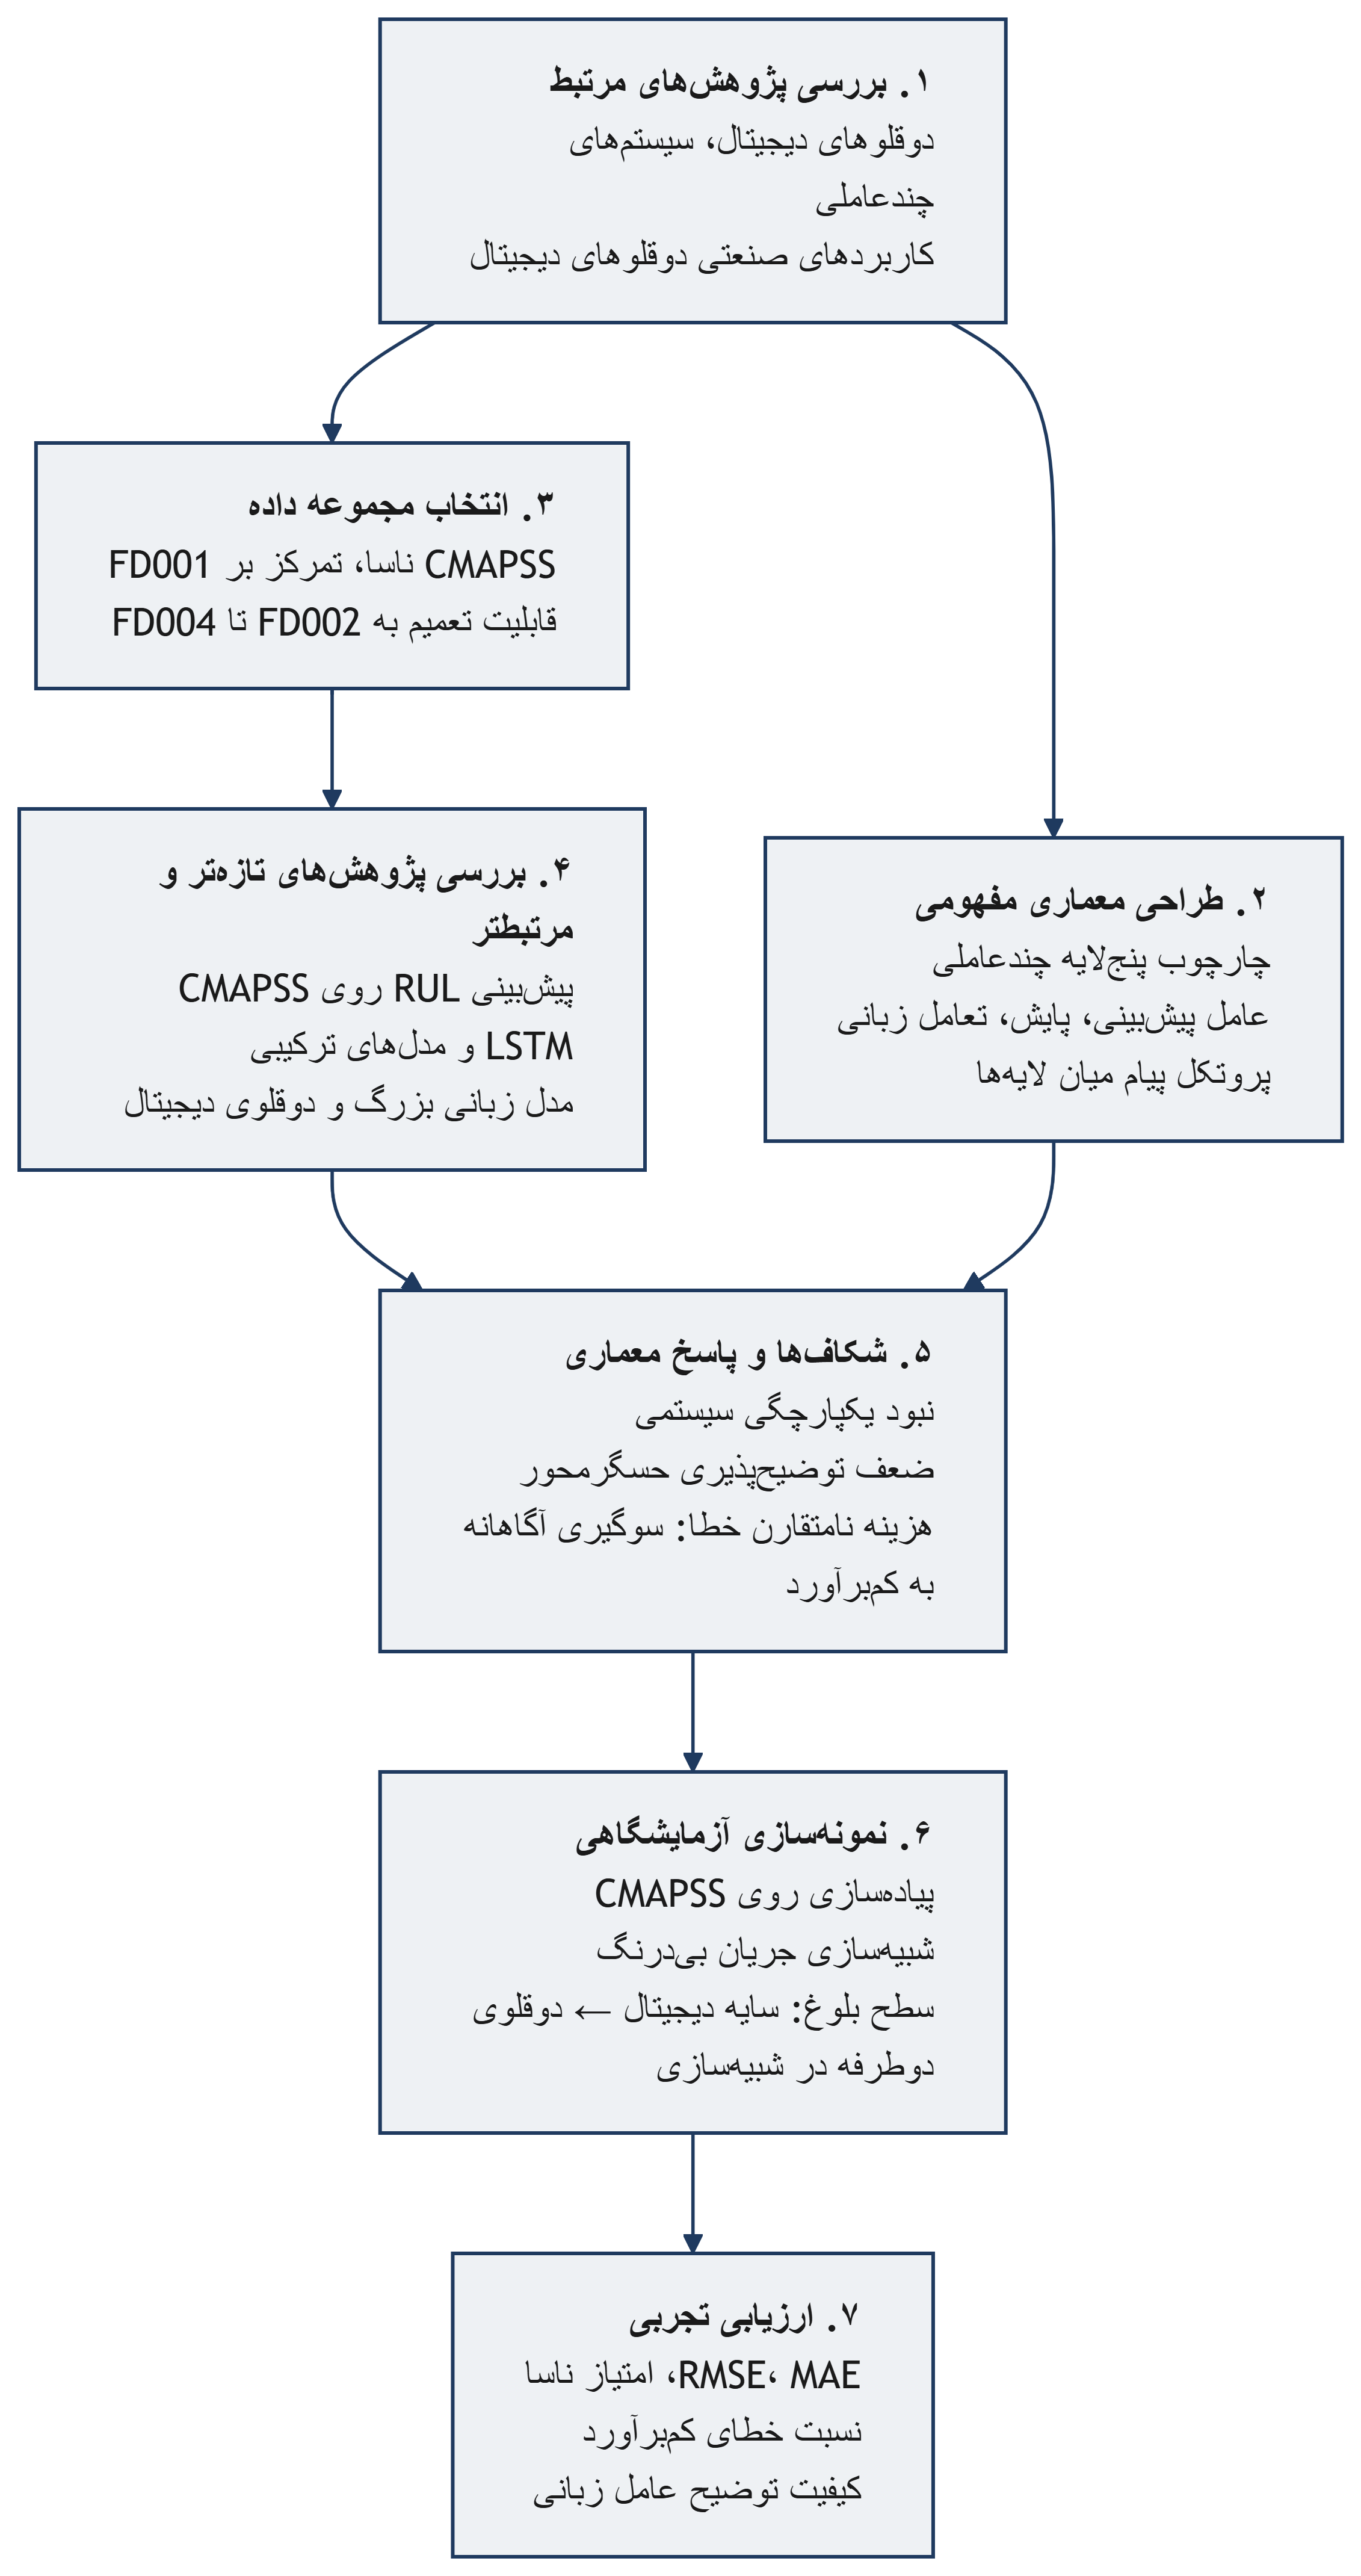
\includegraphics[width=0.8\textwidth]{images/method_flow.png}
	\caption{مسیر هفت‌مرحله‌ای پژوهش: دو شاخه موازی پس از مرور ادبیات --- انتخاب داده و مرور تخصصی در برابر طراحی معماری --- در شناسایی شکاف‌ها به هم می‌رسند و به نمونه‌سازی و ارزیابی می‌انجامند.}
	\label{fig:method-flow}
\end{figure}


% -----------------------------------------------------------------------
\section{معماری پیشنهادی دوقلوی دیجیتال چندعاملی}\label{sec:architecture}

\subsection{نمای کلی و اصول طراحی}\label{sec:arch-overview}

معماری پیشنهادی این پژوهش، چارچوبی پنج‌لایه برای پیاده‌سازی \gls{MA-DT} در سامانه‌های صنعتی است. هر لایه مسئولیتی مشخص و مستقل دارد و از طریق قراردادهای پیام استاندارد با لایه‌های مجاور در ارتباط است. این طراحی بر سه اصل استوار است:

\begin{enumerate}
	\item \textbf{جداسازی مسئولیت‌ها}: هر لایه وظیفه‌ای مشخص دارد و منطق آن با لایه‌های دیگر درهم نمی‌آمیزد. این اصل امکان توسعه، آزمایش و جایگزینی مستقل هر بخش را فراهم می‌کند \cite{wang2024multiagent}.
	\item \textbf{استقلال و همکاری عامل‌ها}: هر عامل به‌صورت خودمختار عمل می‌کند، اما از طریق رابط‌های تعریف‌شده با سایر عامل‌ها همکاری می‌کند \cite{dorri2018multiagent,pretel2022masdt}.
	\item \textbf{مقیاس‌پذیری}: افزودن قابلیت جدید به سامانه تنها نیازمند تعریف عامل جدید در لایه کاربرد است، بدون تغییر در لایه‌های پایین‌تر.
\end{enumerate}

شکل \ref{fig:arch-5layers} نمای کلی این معماری پنج‌لایه را نشان می‌دهد. جریان داده از لایه‌های پایین به بالا --- از موجودیت فیزیکی تا عامل‌های کاربردی --- و جریان فرمان‌ها و بازخوردها در جهت معکوس برقرار است.

\begin{figure}[H]
	\centering
	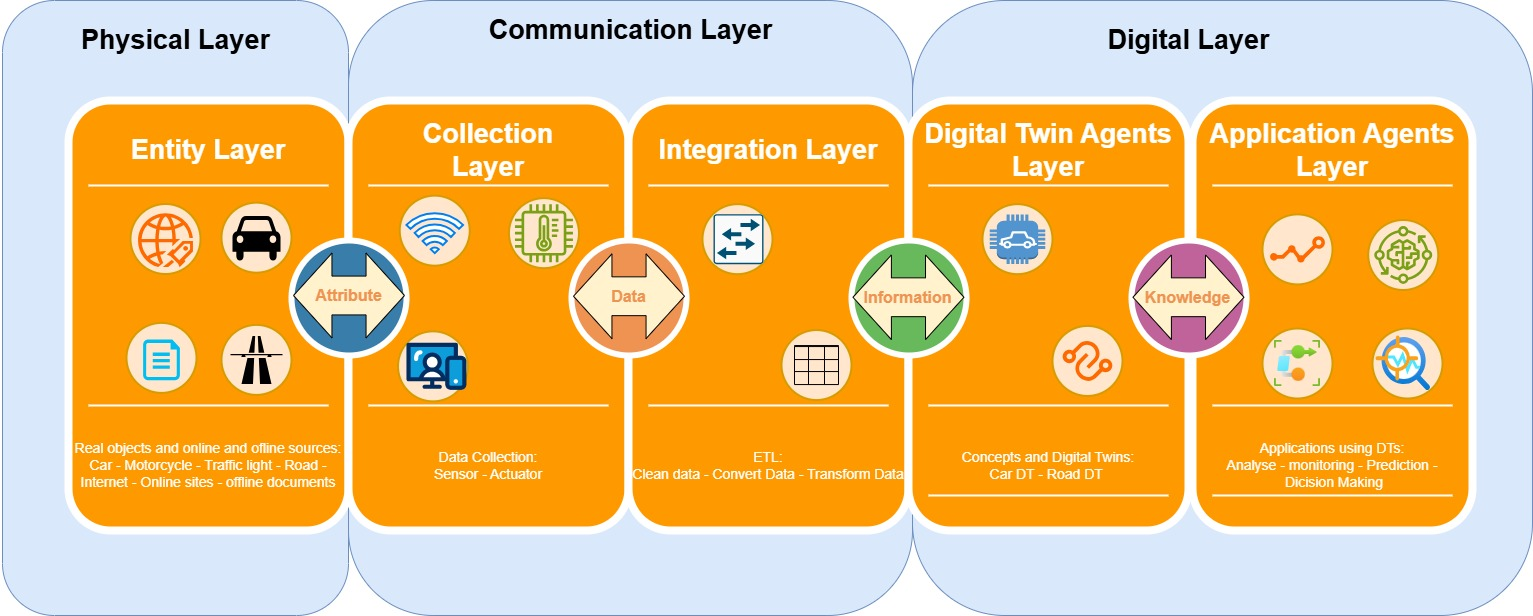
\includegraphics[width=0.98\textwidth]{images/DigitalTwin-Page-4.jpg}
	\caption{معماری پنج‌لایه پیشنهادی \gls{MA-DT}؛ جریان داده از لایه موجودیت به لایه کاربرد صعودی و جریان فرمان‌ها نزولی است \cite{han2025masllmcmapss,park2025interactive.}}
	\label{fig:arch-5layers}
\end{figure}


\subsection{لایه موجودیت}\label{sec:layer-entity}

\gls{EmtityLayer} پایه‌ترین لایه معماری است که موجودیت فیزیکی واقعی را نمایندگی می‌کند. این لایه بر سه مؤلفه اصلی متکی است که پیشتر در فصل دوم معرفی شدند \cite{tao2019digital}:

\begin{itemize}
	\item \textbf{\gls{Physical Entity}}: تجهیز یا فرآیند واقعی که داده‌های حسگری از آن جمع‌آوری می‌شود. در این پژوهش، موجودیت فیزیکی \glspl{Turbofan} است که رفتار تخریبشان توسط مجموعه داده \gls{CMAPSS} ناسا شبیه‌سازی شده است.
	\item \textbf{\gls{Digital Model}}: بازنمایی دیجیتال و محاسباتی از موجودیت فیزیکی که وضعیت لحظه‌ای آن را در حافظه سامانه نگه می‌دارد.
	\item \textbf{\gls{Data Connection}}: مسیر ارتباطی دوطرفه که تبادل داده میان فضای فیزیکی و دیجیتال را ممکن می‌سازد.
\end{itemize}

محدودیت مهم در پژوهش حاضر آن است که داده‌های حسگری واقعی صنعتی در دسترس نیست؛ از این رو موجودیت فیزیکی با موتورهای شماره‌گذاری‌شده در زیرمجموعه‌های \lr{FD001}–\lr{FD004} مجموعه داده \gls{CMAPSS} شبیه‌سازی می‌شود \cite{NASA2007C-MAPSS}.


\subsection{لایه جمع‌آوری داده}\label{sec:layer-collection}

\gls{DataCollectionLayer} مسئول دریافت، نمونه‌برداری و ارسال داده‌های خام حسگرها به لایه‌های بالاتر است. در سامانه‌های صنعتی واقعی، این لایه معمولا از طریق پروتکل‌های \gls{IoT} به تجهیزات متصل می‌شود. در پژوهش حاضر، با خواندن دوره‌ای ردیف‌های مجموعه داده \gls{CMAPSS} و ارسال آن‌ها به‌صورت جریان چرخه ‌به ‌چرخه، این لایه شبیه‌سازی می‌شود.

وظایف اصلی این لایه عبارت‌اند از:
\begin{itemize}
	\item نمونه‌برداری منظم از اندازه‌گیری‌های عملیاتی و خواندن مقادیر حسگرها در هر چرخه کاری.
	\item قرار دادن داده‌ها در صف برای مقاومت در برابر از دست رفتن داده‌ها در صورت تأخیر در پردازش.
	\item جداسازی کامل وظیفه جمع‌آوری از تحلیل، به‌گونه‌ای که این لایه صرفاً داده ارسال می‌کند و هیچ استنتاجی انجام نمی‌دهد.
\end{itemize}


\subsection{لایه ادغام}\label{sec:layer-integration}

\gls{IntegrationLayer} داده‌های خام دریافت‌شده را پردازش و یکپارچه می‌کند تا در قالبی استاندارد برای لایه‌های بالاتر آماده شوند. این لایه سه مسئولیت اصلی دارد:

\begin{enumerate}
	\item \textbf{\gls{Normalization}}: هنجارسازی مقادیر حسگرها به بازه مشخص برای یکپارچگی مقیاس ویژگی‌ها و بهبود همگرایی مدل.
	\item \textbf{تمیزسازی}: تمیز‌سازی داده‌های دریافت شده شامل حذف داده‌های بی‌اعتبار، یکسان‌سازی قالب داده‌ها و آماده استفاده شدن داده‌ها.
	\item \textbf{ساخت پنجره زمانی}: تجمیع داده‌های چند چرخه متوالی برای ساخت توالی ورودی مدل \gls{LSTM}.
	\item \textbf{انتشار وضعیت}: ارسال وضعیت یکپارچه موتور --- شامل شناسه، شماره چرخه، مقادیر هنجارشده حسگرها و آخرین پیش‌بینی \gls{RUL} --- به لایه عامل‌های دوقلوی دیجیتال.
	
	
\end{enumerate}

قرارداد داده در خروجی این لایه به‌صورت ساختاری استاندارد تعریف می‌شود به گونه‌ای که عامل‌ها در لایه دیجیتال بتوانند از آن استفاده کنند.


\subsection{لایه عامل‌های دوقلوی دیجیتال}\label{sec:layer-dt-agents}

\gls{DigitalTwinAgentsLayer} هسته دیجیتالی سامانه را تشکیل می‌دهد. عامل‌های این لایه وضعیت زنده هر موتور را نگه می‌دارند و به‌عنوان نمایندگان دیجیتال موجودیت‌های فیزیکی عمل می‌کنند \cite{marah2024madtwin,tao2018digital}.

ویژگی‌های اصلی این لایه عبارت‌اند از:
\begin{itemize}
	\item \textbf{حالت زنده موتور} (\lr{Twin State}): هر عامل وضعیت آخرین لحظه موتور خود --- شامل چرخه جاری، آخرین \gls{RUL} پیش‌بینی‌شده و وضعیت \gls{Monitoring} --- را در حافظه نگه می‌دارد.
	\item \textbf{به‌روزرسانی پیوسته}: با هر دوره داده جدید از لایه ادغام، وضعیت دیجیتال موتور به‌روز می‌شود.
	\item \textbf{رابط خواندنی}: لایه کاربرد از طریق رابط برنامه‌نویسی می‌تواند وضعیت هر موتور را پرس‌وجو کند درحالی که منطق پیش‌بینی سنگین در این لایه قرار نمی‌گیرد.
\end{itemize}

در این پژوهش، هر موتور در مجموعه داده \gls{CMAPSS} توسط یک عامل مستقل در این لایه نمایندگی می‌شود. این رویکرد از اصل جداسازی مسئولیت‌ها پشتیبانی می‌کند و امکان پایش موازی چند موتور را فراهم می‌آورد \cite{pretel2022masdt,wang2024multiagent}.


\subsection{لایه عامل‌های کاربرد}\label{sec:layer-app-agents}

\gls{ApplicationAgentsLayer} بالاترین لایه معماری چندعاملی دوقلوی دیجیتال است. این لایه محل استقرار خدمات کاربردی و منطق تصمیم است، نه محل نگه‌داری حالت زنده موجودیت. عامل‌های کاربرد وضعیت یکپارچه را از \gls{DigitalTwinAgentsLayer} می‌خوانند، آن را برای هدفی مشخص پردازش می‌کنند و در صورت نیاز فرمان یا بازخورد را به لایه‌های پایین‌تر برمی‌گردانند \cite{wang2024multiagent,pretel2022masdt}. ترکیب عامل‌های این لایه وابسته به دامنه مسئله است و معماری، مجموعه ثابتی از نقش‌ها را تحمیل نمی‌کند.

ویژگی‌های اصلی این لایه، مستقل از مسئله و دادهٔ خاص، عبارت‌اند از:
\begin{itemize}
	\item \textbf{جداسازی منطق کاربرد از داده}: جمع‌آوری، هنجارسازی و نگه‌داری وضعیت زنده در لایه‌های پایین‌تر انجام می‌شود؛ این لایه تنها از قرارداد وضعیت استفاده می‌کند.
	\item \textbf{استقلال و تخصص نقش‌ها}: هر عامل کاربرد مسئول یک خدمت مشخص است --- مانند پیش‌بینی، پایش، بهینه‌سازی، زمان‌بندی نگهداری یا تعامل با کاربر --- و با عامل‌های دیگر از طریق پیام همکاری می‌کند \cite{dorri2018multiagent}.
	\item \textbf{مقیاس‌پذیری}: افزودن قابلیت جدید با تعریف عامل تازه در همین لایه ممکن است، بدون تغییر در لایه‌های موجودیت، جمع‌آوری، ادغام یا دوقلوی دیجیتال.
	\item \textbf{تعامل انسان و فرمان نزولی}: این لایه نقطه اتصال کاربر با سامانه است. درخواست‌ها و دستورهای سطح‌بالا از اینجا به وضعیت دوقلوی دیجیتال و در حالت ایده‌آل به موجودیت فیزیکی منتقل می‌شوند \cite{park2025interactive,CHEN2025102982LLMDT}.
\end{itemize}

در پژوهش حاضر، برای مسئله پیش‌بینی \gls{RUL} روی \gls{CMAPSS} چهار عامل در این لایه در نظر گرفته شده است. این مجموعه مصداق طراحی برای همین مسئله است، نه تعریف عام همه نقش‌های ممکن لایه کاربرد. جزئیات طراحی هر عامل در بخش~\ref{sec:arch-cmapss} آمده است؛ در اینجا تنها نقش انتزاعی آن‌ها معرفی می‌شود:

\begin{enumerate}
	\item \textbf{عامل پیش‌بینی \gls{RUL}}: با دریافت توالی داده‌های حسگری از لایه ادغام، عمر مفید باقیمانده هر موتور را از طریق شبکه \gls{LSTM} آموزش‌دیده پیش‌بینی می‌کند \cite{heimes2008recurrent,zhao2025cmapsslstm}.
	\item \textbf{عامل \gls{Monitoring}}: وضعیت سلامت هر موتور را بر اساس مقدار \gls{RUL} پیش‌بینی‌شده و نرخ افت آن طبقه‌بندی می‌کند و در صورت لزوم هشدار صادر می‌کند.
	\item \textbf{عامل تعامل زبانی}: از طریق \glspl{LLM} رابط زبان طبیعی را برای کاربران فراهم می‌کند و پرسش‌ها را به فراخوان‌های سرویس لایه‌های پایین‌تر ترجمه می‌کند \cite{CHEN2025102982LLMDT,park2025interactive}.
	\item \textbf{عامل شبیه‌سازی جریان داده}: در محیط آزمایشگاهی، جریان داده بی‌درنگ حسگرها را با خواندن دوره‌ای داده‌های \gls{CMAPSS} شبیه‌سازی می‌کند.
\end{enumerate}


\subsection{جریان تعامل و پروتکل ارتباطی}\label{sec:arch-interaction}

جریان اطلاعات در معماری پیشنهادی در دو مسیر اصلی سازمان یافته است:

\textbf{جریان داده صعودی}: داده‌های خام حسگرها از \gls{EmtityLayer} وارد \gls{DataCollectionLayer} می‌شوند، در \gls{IntegrationLayer} پردازش و هنجارسازی می‌شوند. وضعیت دیجیتال موتور در \gls{DigitalTwinAgentsLayer} به‌روز می‌گردد و در نهایت عامل‌های \gls{ApplicationAgentsLayer} وضعیت را پردازش کرده و خروجی تولید می‌کنند.

\textbf{جریان فرمان نزولی}: عامل تعاملی پس از دریافت دستور کاربر --- مثلاً درخواست پیش‌بینی یا فرمان شبیه‌سازی توقف موتور --- آن را از طریق \gls{DigitalTwinAgentsLayer} به لایه‌های پایین‌تر منتقل می‌کند. این ساختار ارتباط \gls{Bidirectional} میان سطوح مختلف سامانه را محقق می‌سازد \cite{tao2019digital}.

شکل \ref{fig:arch-sequence} توالی تعامل عامل‌ها را برای سناریوی نمونه «پیش‌بینی \gls{RUL} موتور $k$ توسط کاربر» نشان می‌دهد.

\begin{figure}[H]
	\centering
	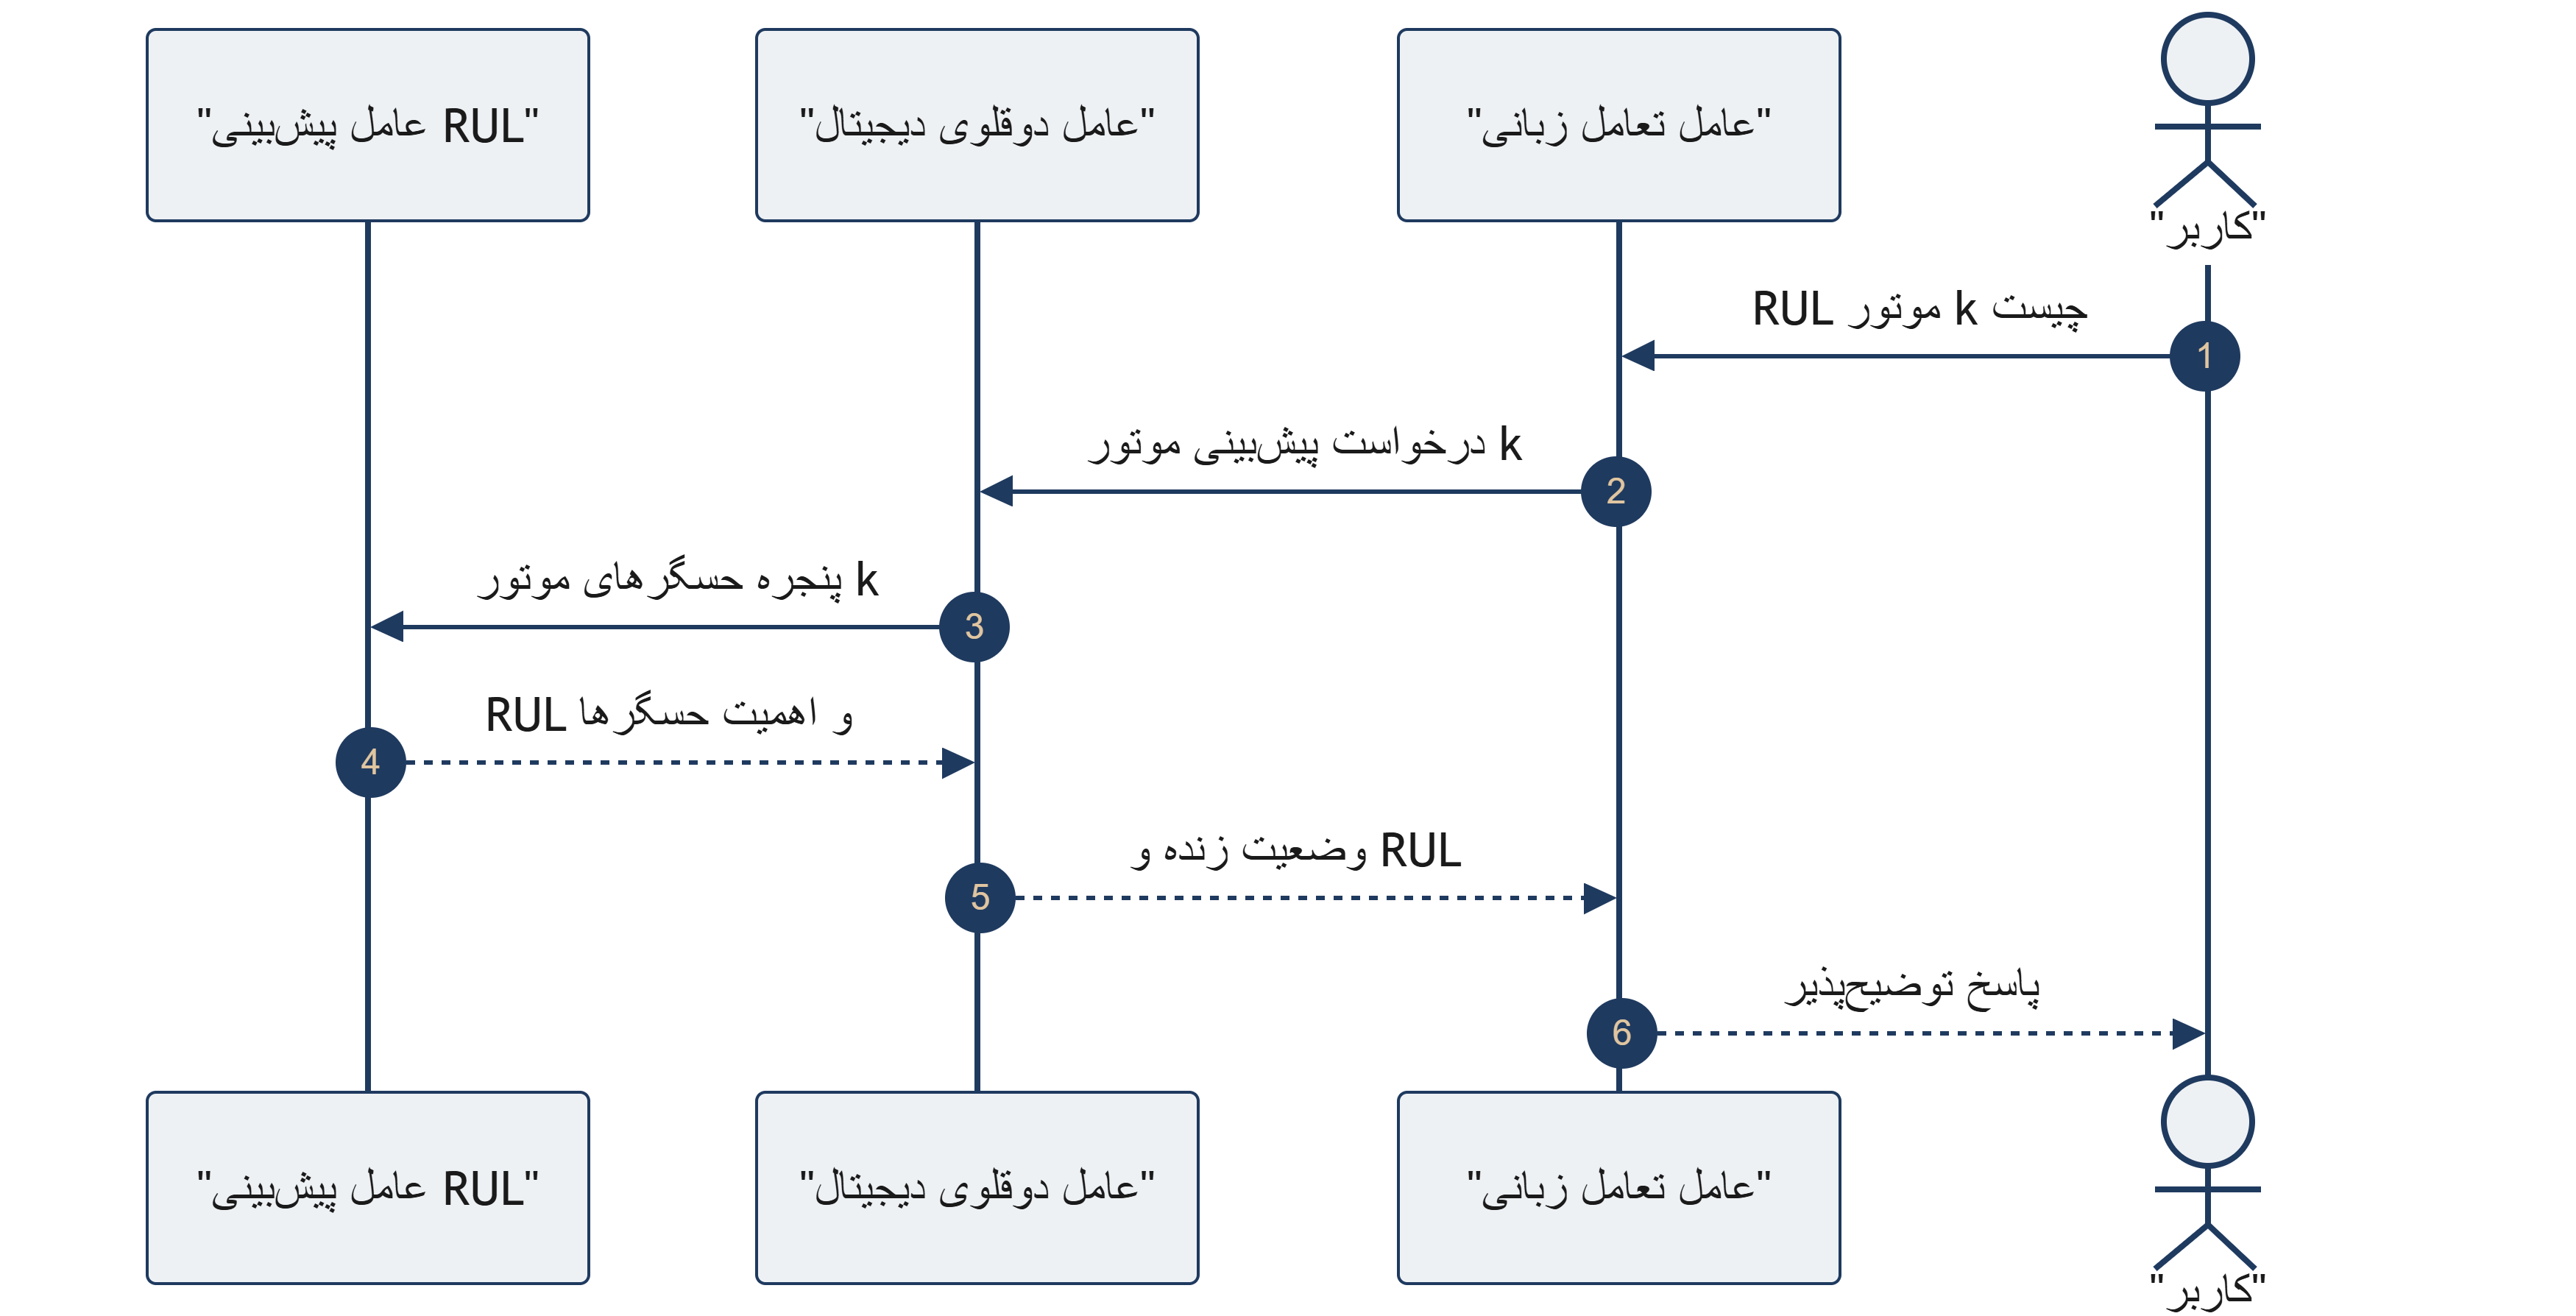
\includegraphics[width=0.92\textwidth]{images/arch_sequence.png}
	\caption{دیاگرام توالی تعامل عامل‌ها برای پرس‌وجوی پیش‌بینی \gls{RUL} از طریق عامل \gls{LLM} \cite{han2025masllmcmapss}}
	\label{fig:arch-sequence}
\end{figure}


% -----------------------------------------------------------------------
\section{مجموعه داده \lr{CMAPSS} و آماده‌سازی داده}\label{sec:dataset}

\subsection{معرفی و ساختار}\label{sec:dataset-intro}

مجموعه داده \gls{CMAPSS} یکی از معتبرترین و پرکاربردترین مجموعه‌های داده در حوزه پیش‌بینی \gls{RUL} تجهیزات صنعتی است که توسط مرکز پژوهش‌های \lr{Glenn} ناسا منتشر شده است \cite{NASA2007C-MAPSS}. این مجموعه داده رفتار تخریب \glspl{Turbofan} را از طریق یک شبیه‌ساز ترموهیدرولیکی مدل می‌کند و در بیش از هزار پژوهش برای ارزیابی الگوریتم‌های پیش‌گویی خرابی به‌کار رفته است \cite{heimes2008recurrent,smith2025cmapsslinear}.

این مجموعه داده شامل چهار زیرمجموعه \lr{FD001} تا \lr{FD004} است که از نظر تعداد شرایط عملیاتی و حالت‌های خرابی با یکدیگر متفاوت‌اند. مشخصات این زیرمجموعه‌ها در جدول \ref{tab:cmapss-subsets} آمده است.

\begin{table}[ht]
	\centering
	\caption{مشخصات زیرمجموعه‌های مجموعه داده \gls{CMAPSS} \cite{NASA2007C-MAPSS}}
	\label{tab:cmapss-subsets}
	\begin{tabular}{ccccc}
		\toprule
		\textbf{زیرمجموعه} & \textbf{شرایط عملیاتی} & \textbf{حالت خرابی} & \textbf{موتور آموزش} & \textbf{موتور آزمون} \\
		\midrule
		\lr{FD001} & ۱ & ۱ & ۱۰۰ & ۱۰۰ \\
		\lr{FD002} & ۶ & ۱ & ۲۶۰ & ۲۵۹ \\
		\lr{FD003} & ۱ & ۲ & ۱۰۰ & ۱۰۰ \\
		\lr{FD004} & ۶ & ۲ & ۲۴۸ & ۲۴۸ \\
		\bottomrule
	\end{tabular}
\end{table}

هر ردیف داده شامل ۲۶ ستون است: شناسه موتور (\lr{unit\_number})، شماره چرخه کاری (\lr{time\_in\_cycles})، سه تنظیم عملیاتی --- ارتفاع، عدد ماخ و زاویه دریچه گاز --- و خوانش ۲۱ حسگر. پژوهش حاضر برای آزمایش اصلی بر زیرمجموعه \lr{FD001} متمرکز است؛ این زیرمجموعه با داشتن یک شرایط عملیاتی و یک حالت خرابی، ارزیابی دقیق‌تری از عملکرد مدل را بدون درهم‌آمیختگی متغیرها ممکن می‌سازد. معماری پیشنهادی به‌گونه‌ای طراحی شده که بدون تغییر ساختاری به زیرمجموعه‌های دیگر نیز تعمیم می‌یابد.

حجم داده به‌کاررفته از \lr{FD001} در جدول \ref{tab:fd001-size} آمده است. داده آموزشی در فایل \lr{train\_FD001.txt} شامل ۲۰۶۳۱ نمونه از ۱۰۰ موتور است که هر موتور تا لحظه خرابی دنبال شده است؛ بیشینه طول عمر در این بخش ۳۶۲ چرخه است. داده آزمون در فایل \lr{test\_FD001.txt} شامل ۱۳۰۹۶ نمونه از ۱۰۰ موتور است که دنباله هر موتور پیش از خرابی قطع می‌شود؛ بیشینه چرخه مشاهده‌شده در آزمون ۳۰۳ است \cite{NASA2007C-MAPSS}.

\begin{table}[ht]
	\centering
	\caption{حجم داده به‌کاررفته از زیرمجموعه \lr{FD001}}
	\label{tab:fd001-size}
	\begin{tabular}{cccc}
		\toprule
		\textbf{بخش} & \textbf{تعداد موتور} & \textbf{تعداد نمونه} & \textbf{بیشینه چرخه} \\
		\midrule
		آموزش & ۱۰۰ & ۲۰۶۳۱ & ۳۶۲ \\
		آزمون & ۱۰۰ & ۱۳۰۹۶ & ۳۰۳ \\
		\bottomrule
	\end{tabular}
\end{table}


\subsection{چالش‌های داده}\label{sec:dataset-challenges}

کار با مجموعه داده \gls{CMAPSS} با چند چالش همراه است که روش‌شناسی پژوهش حاضر را شکل می‌دهد:

\begin{itemize}
	\item \textbf{ستون‌های بی‌اطلاع}: بخشی از حسگرها و تنظیم‌های عملیاتی در \lr{FD001} واریانس صفر یا نزدیک به صفر دارند و هیچ اطلاعاتی از وضعیت تخریب حمل نمی‌کنند. نگه‌داشتن این ستون‌ها به آموزش مدل آسیب می‌زند و حذف آن‌ها را ضروری می‌کند.
	\item \textbf{هم‌خطی میان حسگرها}: برخی حسگرها با یکدیگر همبستگی بسیار بالا دارند و اطلاعات تکراری وارد مدل می‌کنند؛ نمونه بارز آن جفت \lr{Nc} و \lr{NRc} است.
	\item \textbf{طول عمر متغیر}: طول عمر موتورهای آموزشی تا ۳۶۲ چرخه می‌رسد و از موتوری به موتور دیگر متفاوت است. این اختلاف، ساخت توالی با طول ثابت و در صورت نیاز تکمیل ابتدای دنباله‌های کوتاه را الزامی می‌کند.
	\item \textbf{هزینه نامتقارن خطا}: در سناریوی \gls{predictive maintenance}، بیش‌برآورد \gls{RUL} به‌مراتب زیان‌بارتر از کم‌برآورد آن است \cite{nguyen2025underestimate}. اگر مدل عمر باقیمانده موتوری را بیشتر از واقعیت برآورد کند، نگهداری به تأخیر می‌افتد و احتمال خرابی ناگهانی و پرهزینه افزایش می‌یابد. از این رو طراحی تابع هزینه در پژوهش حاضر به‌گونه‌ای است که خطاها را آگاهانه به سمت کم‌برآورد سوق می‌دهد؛ موضوعی که در بخش~\ref{sec:lstm-design} به‌تفصیل توضیح داده می‌شود.
\end{itemize}


\subsection{تحلیل اکتشافی و انتخاب ویژگی}\label{sec:eda}

آماده‌سازی داده با آمار توصیفی ستون‌ها و سپس تحلیل همبستگی آغاز می‌شود. آمار توصیفی نشان می‌دهد که هفت ستون در کل داده آموزشی مقدار ثابت دارند: \lr{TRA}، \lr{T2}، \lr{P2}، \lr{epr}، \lr{farB}، \lr{Nf\_dmd} و \lr{PCNfR\_dmd}. این ستون‌ها پیش از ساخت برچسب حذف می‌شوند.

پس از محاسبه برچسب \gls{RUL}، همبستگی پیرسون میان ویژگی‌های باقی‌مانده و هدف به‌دست می‌آید. شکل \ref{fig:corr-heatmap} این نقشه همبستگی را نشان می‌دهد. همبستگی \lr{RUL} با \lr{time\_in\_cycles}، \lr{Ps30}، \lr{T50} و \lr{BPR} منفی و نسبتاً قوی است؛ با \lr{phi}، \lr{W31} و \lr{W32} مثبت و قابل‌توجه است. در مقابل، \lr{setting\_1} و \lr{setting\_2} همبستگی نزدیک به صفر با هدف دارند و همبستگی \lr{P15} نیز ضعیف است. همچنین همبستگی میان \lr{Nc} و \lr{NRc} برابر ۰٫۹۶ است و نگه‌داشتن هر دو ویژگی اطلاعات تکراری ایجاد می‌کند.

% منبع شکل: سلول sns.heatmap در Implementation/jupyter-notebook/main_lstm_1.ipynb
\begin{figure}[H]
	\centering
	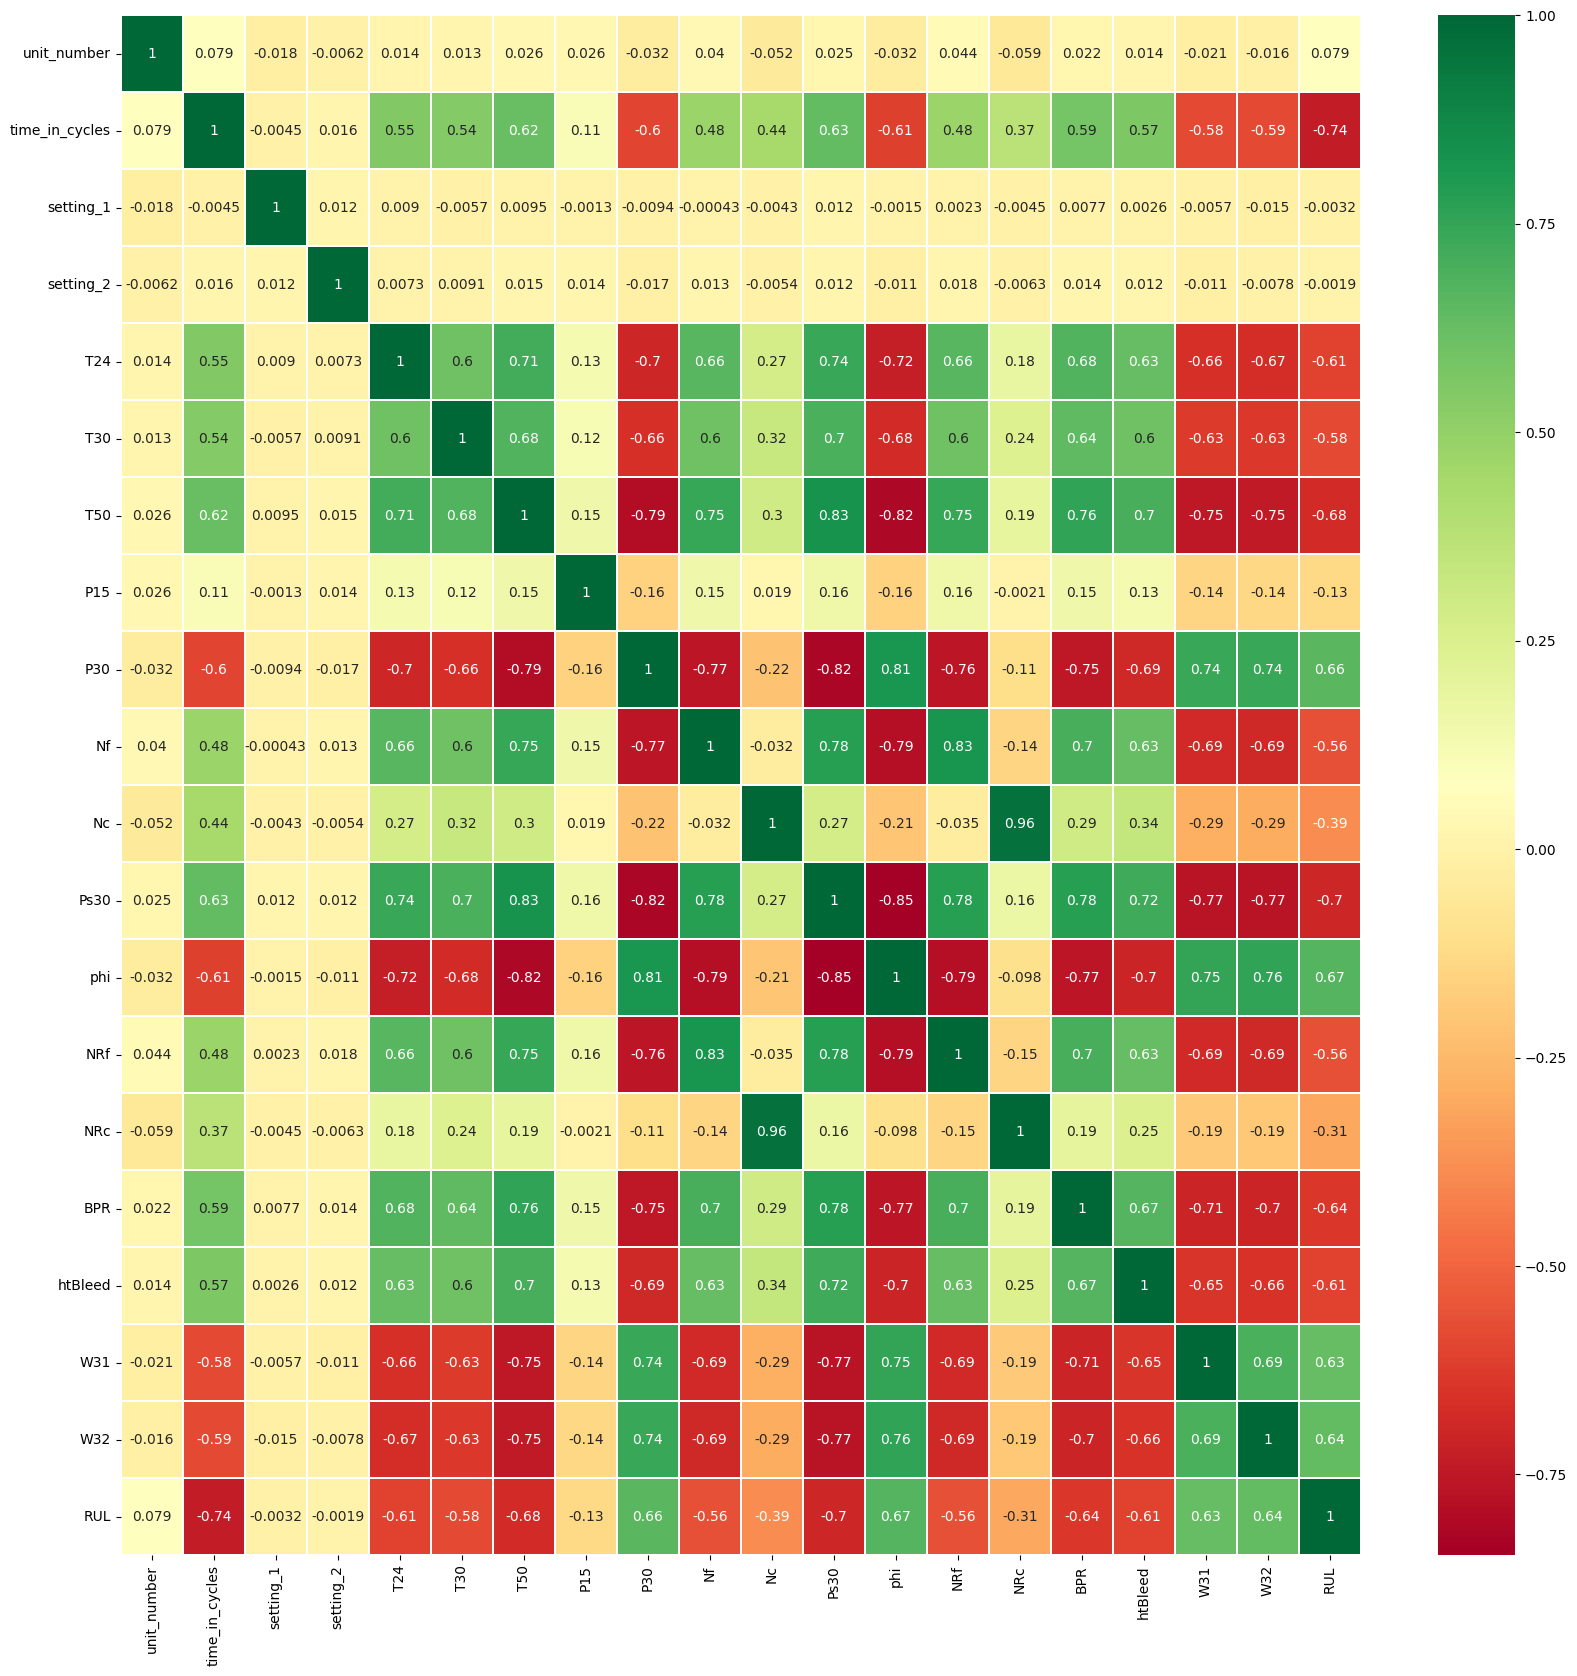
\includegraphics[width=0.98\textwidth]{images/cmapss_corr_heatmap.png}
	\caption{نقشه همبستگی پیرسون ویژگی‌ها و برچسب \gls{RUL} در داده آموزشی \lr{FD001} پس از حذف ستون‌های ثابت}
	\label{fig:corr-heatmap}
\end{figure}

بر این اساس، انتخاب ویژگی در دو گام انجام می‌شود و نتیجه آن در جدول \ref{tab:feature-selection} آمده است. گام نخست حذف ستون‌های ثابت است. گام دوم حذف تنظیم‌های عملیاتی کم‌اطلاع، حسگر \lr{P15} و حسگر تکراری \lr{NRc} است. سیزده حسگر باقی‌مانده به‌همراه شماره چرخه، ورودی مراحل بعدی را می‌سازند. شناسه موتور برای تفکیک توالی هر واحد نگه داشته می‌شود و به‌عنوان ویژگی فیزیکی به‌کار نمی‌رود.

\begin{table}[ht]
	\centering
	\caption{مراحل انتخاب ویژگی در زیرمجموعه \lr{FD001}}
	\label{tab:feature-selection}
	\begin{tabular}{p{3.6cm}p{9.2cm}}
		\toprule
		\textbf{گام} & \textbf{ستون‌ها} \\
		\midrule
		حذف ستون‌های ثابت & \lr{TRA}، \lr{T2}، \lr{P2}، \lr{epr}، \lr{farB}، \lr{Nf\_dmd} و \lr{PCNfR\_dmd} \\
		حذف همبستگی ضعیف یا تکراری & \lr{setting\_1}، \lr{setting\_2}، \lr{P15} و \lr{NRc} \\
		حسگرهای منتخب & \lr{T24}، \lr{T30}، \lr{T50}، \lr{P30}، \lr{Nf}، \lr{Nc}، \lr{Ps30}، \lr{phi}، \lr{NRf}، \lr{BPR}، \lr{htBleed}، \lr{W31} و \lr{W32} \\
		\bottomrule
	\end{tabular}
\end{table}


\subsection{پیش‌پردازش داده}\label{sec:preprocessing}

پس از تمیزسازی و انتخاب ویژگی، داده برای آموزش مدل \gls{LSTM} به توالی هنجارشده تبدیل می‌شود. مراحل این تبدیل به شرح زیر است.

\textbf{برچسب‌گذاری \gls{RUL}}: برچسب در داده آموزشی به‌صورت آشکار موجود نیست و از روی دنباله هر موتور محاسبه می‌شود. اگر $t^{(i)}_{\mathrm{end}}$ آخرین چرخه موتور $i$ باشد --- یعنی لحظه خرابی --- مقدار \gls{RUL} در چرخه $t$ برابر است با

\begin{equation}\label{eq:rul-label}
y^{(i)}(t) = t^{(i)}_{\mathrm{end}} - t.
\end{equation}

مقدار رابطه \eqref{eq:rul-label} به‌عنوان هدف رگرسیون به‌کار می‌رود. در داده آزمون، دنباله پیش از خرابی قطع شده است؛ بنابراین مقدار باقیمانده واقعی از فایل \lr{RUL\_FD001.txt} خوانده می‌شود. اگر $t^{(i)}_{\mathrm{last}}$ آخرین چرخه مشاهده‌شده در آزمون و $y^{(i)}_{\mathrm{file}}$ مقدار همان فایل باشد،

\begin{equation}\label{eq:rul-test}
y^{(i)}(t) = t^{(i)}_{\mathrm{last}} + y^{(i)}_{\mathrm{file}} - t.
\end{equation}

بدین ترتیب، برچسب در آخرین چرخه آزمون با مقدار فایل ناسا یکی است \cite{NASA2007C-MAPSS}.

\textbf{\gls{Normalization}}: مقادیر حسگرهای منتخب با هنجارسازی \lr{Min-Max} به بازه $[0, 1]$ تبدیل می‌شوند:

\begin{equation}\label{eq:normalization}
x_{\mathrm{norm}} = \frac{x - x_{\min}}{x_{\max} - x_{\min}}.
\end{equation}

پارامترهای $x_{\min}$ و $x_{\max}$ فقط از داده آموزشی برآورد می‌شوند و همان تبدیل روی داده آزمون اعمال می‌گردد تا از نشت اطلاعات جلوگیری شود. شناسه موتور، شماره چرخه خام و برچسب \gls{RUL} از این تبدیل مستثنا هستند. نسخه هنجارشده شماره چرخه در ستون جداگانه‌ای با نام \lr{cycle\_norm} ذخیره می‌شود و همراه حسگرهای منتخب در پنجره زمانی قرار می‌گیرد.

% در نوت‌بوک‌های jupyter-notebook نمودار سری زمانی یک حسگر پیش و پس از هنجارسازی موجود نیست.
% در صورت نیاز، در main_lstm_1.ipynb برای یک موتور آموزشی نمونه (مثلاً حسگرهای T50 یا Ps30) سری زمانی خام و هنجارشده رسم و با نام images/cmapss_sensor_norm.png ذخیره شود؛ سپس شکل زیر فعال گردد:
% \begin{figure}[H]
%	\centering
%	\includegraphics[width=0.85\textwidth]{images/cmapss_sensor_norm.png}
%	\caption{سری زمانی نمونه یک حسگر از موتور آموزشی \lr{FD001}؛ پیش و پس از هنجارسازی \lr{Min-Max}}
%	\label{fig:sensor-timeseries}
% \end{figure}

\textbf{ساخت توالی}: ورودی شبکه \gls{LSTM} پنجره‌ای لغزنده به طول $w=50$ چرخه است. برای هر موتور، از ابتدای دنباله تا انتها پنجره‌های متوالی ساخته می‌شود و برچسب هر پنجره برابر \gls{RUL} آخرین گام آن پنجره است. اگر طول دنباله واحدی کمتر از ۵۰ چرخه باشد --- وضعیتی که در برخی موتورهای آزمون رخ می‌دهد --- ابتدای توالی با صفر پر می‌شود تا ابعاد ورودی ثابت بماند.

\textbf{تقسیم داده}: طبق پروتکل استاندارد \gls{CMAPSS}، تقسیم آموزش و آزمون از پیش در فایل‌ها تعریف شده است و تقسیم تصادفی روی نمونه‌ها انجام نمی‌شود. داده آموزشی توالی کامل تا خرابی است و داده آزمون دنباله‌ای قطع‌شده است \cite{NASA2007C-MAPSS}.


% -----------------------------------------------------------------------
\section{انطباق معماری پیشنهادی بر مسئله \lr{CMAPSS}}\label{sec:arch-cmapss}

این بخش قلب فصل است و نشان می‌دهد که چگونه معماری عمومی پنج‌لایه روی مسئله مشخص پیش‌بینی \gls{RUL} موتورهای \gls{Turbofan} پیاده می‌شود.


\subsection{نگاشت لایه‌ها به اجزای مسئله}\label{sec:layer-mapping}

جدول \ref{tab:layer-mapping} نگاشت هر لایه از معماری پیشنهادی به اجزای مشخص مسئله \gls{CMAPSS} را نشان می‌دهد.

\begin{table}[ht]
	\centering
	\caption{نگاشت لایه‌های معماری پیشنهادی به اجزای مسئله \gls{CMAPSS}}
	\label{tab:layer-mapping}
	\begin{descitemize}
		\item[\gls{EmtityLayer}:] ورودی سیگنال‌های خام حسگر؛ مصداق آن \glspl{Turbofan} شبیه‌سازی‌شده در \lr{FD001} تا \lr{FD004} است.
		\item[\gls{DataCollectionLayer}:] داده چرخه‌ای را به بافر می‌فرستد؛ مصداق آن خواندن ردیف‌به‌ردیف فایل‌های \lr{train\_FD00x.txt} است.
		\item[\gls{IntegrationLayer}:] داده خام را به توالی هنجارشده تبدیل می‌کند؛ شامل هنجارسازی، انتخاب ۱۳ حسگر و ساخت پنجره به طول ۵۰ چرخه.
		\item[\gls{DigitalTwinAgentsLayer}:] توالی را به وضعیت زنده موتور نگاشت می‌کند و وضعیت دوقلو را نگه می‌دارد.
		\item[\gls{ApplicationAgentsLayer}:] وضعیت را به پیش‌بینی، هشدار و پاسخ زبانی تبدیل می‌کند.
	\end{descitemize}
\end{table}


\subsection{طراحی عامل پیش‌بینی عمر مفید باقیمانده}\label{sec:lstm-design}

مسئله پیش‌بینی \gls{RUL} به‌صورت رگرسیون روی توالی‌های زمانی فرموله می‌شود. به‌ازای هر نمونه با توالی ورودی $\mathbf{X} \in \mathbb{R}^{w \times d}$ --- که $w=50$ طول پنجره و $d$ تعداد ویژگی‌های منتخب در هر گام زمانی است --- مدل باید مقدار \gls{RUL} در لحظه $t$ را تخمین بزند.

\textbf{معماری مفهومی شبکه}: شبکه از دو لایه \gls{LSTM} پشت‌سرهم تشکیل می‌شود که خروجی آن از طریق لایه‌های \lr{Dropout} و \lr{Dense} به مقدار \gls{RUL} تبدیل می‌شود. لایه اول \gls{LSTM} کل دنباله را پردازش می‌کند و خروجی آن به لایه دوم می‌رسد که تنها وضعیت آخرین گام زمانی را به لایه \lr{Dense} منتقل می‌کند \cite{heimes2008recurrent}. جزئیات هایپرپارامترها و کد پیاده‌سازی در فصل چهارم آمده است.

\textbf{تابع هزینه ناهم‌تراز}: نوآوری اصلی در طراحی عامل پیش‌بینی، استفاده از تابع هزینه‌ای است که خطا را آگاهانه به سمت کم‌برآورد سوق می‌دهد \cite{nguyen2025underestimate}. این تابع از خاصیت نامتقارن تابع امتیاز ناسا \cite{NASA2007C-MAPSS,heimes2008recurrent} الهام گرفته و برای آموزش شبکه بهینه‌سازی شده است:

\begin{equation}\label{eq:asym-loss}
L(\hat{y},\, y) = w(d)\,(\hat{y} - y)^{2},
\qquad
d = \hat{y} - y.
\end{equation}

وزن $w(d)$ برابر $\alpha$ در بیش‌برآورد ($d>0$) و برابر $\beta$ در کم‌برآورد ($d\leq 0$) است؛ $\hat{y}$ مقدار پیش‌بینی‌شده \gls{RUL} و $y$ مقدار واقعی است. با انتخاب $\alpha > \beta$، جریمه بیش‌برآورد سنگین‌تر از کم‌برآورد تعریف می‌شود. در نتیجه، هنگامی که مدل در شرایط عدم‌قطعیت خطا می‌کند، تمایل دارد مقدار کمتری برآورد کند --- رفتاری که از منظر ایمنی صنعتی محافظه‌کارانه و مطلوب است \cite{nguyen2025underestimate}.

برای ارزیابی جامع‌تر سوگیری خطا، علاوه بر معیارهای استاندارد، از تابع امتیاز ناسا \cite{NASA2007C-MAPSS} نیز استفاده می‌شود:

\begin{equation}\label{eq:nasa-score}
S = \sum_{i=1}^{N} s_i,
\qquad
s_i = e^{|d_{i}|/c_{i}} - 1.
\end{equation}

ضریب $c_i$ برابر $10$ در بیش‌برآورد ($d_i \geq 0$) و برابر $13$ در کم‌برآورد ($d_i < 0$) است. چون مخرج خطای بیش‌برآورد از مخرج خطای کم‌برآورد کوچک‌تر است، این تابع برای بیش‌برآورد جریمه بیشتری اعمال می‌کند؛ خاصیتی هم‌راستا با طراحی تابع هزینه آموزشی رابطه \eqref{eq:asym-loss}.

\textbf{خروجی عامل}: پس از آموزش، عامل پیش‌بینی به‌ازای هر موتور یک مقدار \gls{RUL} تخمینی تولید می‌کند. این مقدار به عامل \gls{Monitoring} و از طریق آن به عامل تعاملی \gls{LLM} ارسال می‌شود.


\subsection{طراحی توضیح‌پذیری و تحلیل سهم حسگرها}\label{sec:explainability}

یکی از شکاف‌های مهم شناسایی‌شده در فصل دوم، غفلت پژوهش‌های پیشین از تحلیل سهم هر حسگر در تصمیم مدل پیش‌بینی است. پژوهش حاضر برای رفع این شکاف، روشی برای شناسایی حسگرهای مؤثر بر پیش‌بینی \gls{RUL} هر موتور طراحی می‌کند \cite{han2025masllmcmapss}.

رویکرد طراحی‌شده مبتنی بر تحلیل حساسیت ورودی است: با اعمال اختلال کوچک به هر ویژگی حسگری در پنجره ورودی و اندازه‌گیری تغییر در خروجی \gls{RUL}، اهمیت نسبی هر حسگر برآورد می‌شود:

\begin{equation}\label{eq:sensitivity}
I_j = \left|\frac{\partial \hat{y}}{\partial x_j}\right|, \qquad j = 1, \ldots, d
\end{equation}

که در آن $I_j$ اهمیت حسگر $j$ام است. بردار اهمیت حسگرها $\mathbf{I} = (I_1, \ldots, I_d)$ به‌همراه مقدار \gls{RUL} به عامل تعامل زبانی ارسال می‌شود تا توضیح‌های انسانی‌خوان تولید کند. نمودارها و نتایج کمی این تحلیل در فصل پنجم ارائه می‌شود.


\subsection{طراحی عامل پایش بی‌درنگ}\label{sec:monitoring-design}

عامل \gls{Monitoring} وظیفه پایش مستمر وضعیت سلامت موتورها و صدور هشدار به‌موقع را بر عهده دارد. این عامل بر اساس مقدار \gls{RUL} دریافت‌شده از عامل پیش‌بینی، وضعیت هر موتور را در یکی از سه حالت زیر طبقه‌بندی می‌کند:

\begin{table}[ht]
	\centering
	\caption{حالت‌های پایش و شرایط انتقال بین آن‌ها}
	\label{tab:monitoring-states}
	\begin{itemize}
		\item \textbf{عادی} ($\mathrm{RUL} > \theta_{\mathrm{warn}}$): ادامه پایش دوره‌ای.
		\item \textbf{هشدار} ($\theta_{\mathrm{crit}} < \mathrm{RUL} \leq \theta_{\mathrm{warn}}$): ارسال رویداد هشدار به عامل \gls{LLM}.
		\item \textbf{بحرانی} ($\mathrm{RUL} \leq \theta_{\mathrm{crit}}$): ارسال هشدار فوری و پیشنهاد توقف.
	\end{itemize}
\end{table}

که در آن $\theta_{\mathrm{warn}}$ و $\theta_{\mathrm{crit}}$ آستانه‌های هشدار و بحران هستند که بر اساس الزامات سناریوی صنعتی تنظیم می‌شوند.

شبیه‌سازی جریان بی‌درنگ در پژوهش حاضر با خواندن چرخه‌به‌چرخه فایل‌های \gls{CMAPSS} و ارسال آن‌ها با تأخیر زمانی شبیه‌سازی‌شده انجام می‌گیرد. این رویکرد رفتار سامانه پایش واقعی را در بستر آزمایشگاهی بازتولید می‌کند \cite{nguyen2025edgedt,marah2024madtwin}.


\subsection{طراحی عامل تعاملی مدل زبانی بزرگ}\label{sec:llm-design}

نقش \gls{LLM} در این معماری به‌عنوان رابط زبان طبیعی تعریف شده، نه جایگزین مدل پیش‌بینی \gls{RUL}. این طراحی با رویکرد \lr{LLM-as-Reasoner} در ادبیات اخیر هم‌راستاست \cite{CHEN2025102982LLMDT,park2025interactive,zhao2025llmmaintenance}.

قابلیت‌های هدف عامل تعاملی عبارت‌اند از:

\begin{enumerate}
	\item \textbf{پرس‌وجوی وضعیت}: کاربر می‌تواند با زبان طبیعی وضعیت سلامت موتور خاصی را بپرسد و عامل از طریق رابط \gls{DigitalTwinAgentsLayer} اطلاعات را دریافت و به زبانی قابل‌فهم بازگو کند.
	\item \textbf{درخواست پیش‌بینی}: کاربر می‌تواند درخواست پیش‌بینی \gls{RUL} موتور مشخصی را بدهد؛ عامل این درخواست را به فراخوان سرویس عامل پیش‌بینی ترجمه می‌کند.
	\item \textbf{توضیح دلیل}: عامل با ترکیب مقدار \gls{RUL} و بردار اهمیت حسگرها (از بخش~\ref{sec:explainability}) توضیحی زبانی تولید می‌کند که نشان می‌دهد کدام حسگرها بیشترین نقش را در پیش‌بینی داشته‌اند.
	\item \textbf{فرمان‌های سطح‌بالا}: کاربر می‌تواند دستوراتی مانند «موتور $k$ را از مدار خارج کن» یا «گزارش موتورهای زیر آستانه بحران را بده» صادر کند.
\end{enumerate}

الگوی طراحی از رویکرد \lr{Tool-Calling} پیروی می‌کند: \gls{LLM} هنگام دریافت درخواست کاربر، یک یا چند ابزار --- سرویس‌های عامل‌های دیگر --- را فراخوانی می‌کند و خروجی آن‌ها را در پاسخ نهایی ترکیب می‌کند. این ساختار مرز ایمنی روشنی ایجاد می‌کند: \gls{LLM} هیچ دسترسی مستقیمی به داده‌های خام یا مدل \gls{LSTM} ندارد و تنها از طریق رابط‌های تعریف‌شده عمل می‌کند \cite{han2025masllmcmapss,CHEN2025102982LLMDT}. جزئیات پیاده‌سازی این الگو از طریق پلتفرم \lr{Dify} در فصل چهارم ارائه می‌شود.


\subsection{همگام‌سازی چندعاملی و سناریوی سرتاسری}\label{sec:e2e-scenario}

برای نشان دادن انسجام معماری، سناریوی سرتاسری زیر طراحی شده است. این سناریو مسیر کامل داده از ورود تا پاسخ توضیح‌پذیر را پوشش می‌دهد:

\begin{enumerate}
	\item \textbf{ورود داده}: عامل شبیه‌سازی، داده چرخه $t$ موتور $k$ را از فایل \gls{CMAPSS} می‌خواند و به \gls{DataCollectionLayer} ارسال می‌کند.
	\item \textbf{پردازش یکپارچه}: \gls{IntegrationLayer} توالی جدید را هنجار می‌کند و پنجره لغزنده را به‌روز می‌کند.
	\item \textbf{به‌روزرسانی دوقلو}: عامل \gls{DigitalTwinAgentsLayer} وضعیت دیجیتال موتور $k$ را به‌روز می‌کند.
	\item \textbf{پیش‌بینی}: عامل پیش‌بینی درخواست دریافت می‌کند، مقدار \gls{RUL} و بردار اهمیت حسگرها را محاسبه و به لایه دوقلو برمی‌گرداند.
	\item \textbf{پایش}: عامل \gls{Monitoring} وضعیت را ارزیابی می‌کند؛ در صورت ورود به حالت هشدار یا بحران، رویداد ارسال می‌شود.
	\item \textbf{تعامل}: کاربر از طریق عامل \gls{LLM} می‌پرسد «چرا \gls{RUL} موتور $k$ کاهش یافته است؟»؛ عامل با ترکیب خروجی‌های مراحل قبل پاسخی توضیح‌پذیر و مبتنی بر حسگرها تولید می‌کند.
\end{enumerate}

دیاگرام توالی این سناریو در شکل \ref{fig:arch-sequence} نشان داده شده است.


% -----------------------------------------------------------------------
\section{روش ارزیابی طراحی‌شده}\label{sec:eval-design}

معیارهای ارزیابی در این بخش تعریف می‌شوند تا فصل پنجم تنها به گزارش نتایج عددی بپردازد.

\subsection*{معیارهای کمی پیش‌بینی}

برای ارزیابی دقت پیش‌بینی \gls{RUL}، سه معیار استاندارد به‌کار می‌رود:

\begin{equation}\label{eq:rmse}
\mathrm{RMSE} = \sqrt{\frac{1}{N}\sum_{i=1}^{N}(\hat{y}_i - y_i)^2}
\end{equation}
\begin{equation}\label{eq:mae}
\mathrm{MAE} = \frac{1}{N}\sum_{i=1}^{N}\left| \hat{y}_i - y_i \right|
\end{equation}
\begin{equation}\label{eq:r2}
R^{2} = 1 - \frac{\sum_{i=1}^{N}(\hat{y}_i - y_i)^2}{\sum_{i=1}^{N}(\bar{y} - y_i)^2}
\end{equation}

علاوه بر معیارهای بالا، تابع امتیاز ناسا (رابطه \eqref{eq:nasa-score}) به‌عنوان معیار اصلی ارزیابی رفتار سوگیری خطا استفاده می‌شود \cite{NASA2007C-MAPSS,heimes2008recurrent}.

\subsection*{معیار اختصاصی سوگیری خطا}

برای تأیید اینکه تابع هزینه ناهم‌تراز (رابطه \eqref{eq:asym-loss}) خطاها را به سمت کم‌برآورد سوق داده است، نسبت خطاهای کم‌برآورد به کل نمونه‌های آزمون محاسبه می‌شود:

\begin{equation}\label{eq:bias-ratio}
r_{\mathrm{under}} = \frac{\left| \{i : \hat{y}_i < y_i\} \right|}{N}
\end{equation}

مقدار $r_{\mathrm{under}} > 0.5$ نشان می‌دهد که سامانه تمایل به کم‌برآورد دارد. این معیار تأیید می‌کند که طراحی تابع هزینه به هدف محافظه‌کارانه خود دست یافته --- نه اینکه مدل دارای ضعف ساختاری باشد.

\subsection*{معیارهای ارزیابی سامانه چندعاملی}

برای ارزیابی جنبه‌های سامانه‌ای فراتر از دقت پیش‌بینی:

\begin{itemize}
	\item \textbf{زمان پاسخ}: میانگین تأخیر از دریافت داده جدید تا تولید خروجی توسط عامل \gls{Monitoring}.
	\item \textbf{صحت فرمان}: درصد فرمان‌های سطح‌بالای کاربر که به‌درستی تفسیر و اجرا می‌شوند.
	\item \textbf{کیفیت توضیح}: ارزیابی کیفی نمونه‌های پاسخ عامل \gls{LLM} از نظر دقت، صحت استناد به حسگرها و روانی.
\end{itemize}

مقایسه عملکرد پیش‌بینی با خطوط پایه ادبیات --- از جمله مدل‌های خطی \cite{smith2025cmapsslinear}، شبکه \gls{Bi-LSTM} \cite{zhao2025cmapsslstm} و مدل ترکیبی \lr{CNN-LSTM} \cite{chang2024hybriddt} --- در فصل پنجم با اعداد و نمودارها ارائه می‌شود.


% -----------------------------------------------------------------------
\section{جمع‌بندی}\label{sec:chap3-summary}

در این فصل روش‌شناسی پژوهش و معماری پیشنهادی \gls{MA-DT} به‌تفصیل ارائه شد. معماری پنج‌لایه --- شامل \gls{EmtityLayer}، \gls{DataCollectionLayer}، \gls{IntegrationLayer}، \gls{DigitalTwinAgentsLayer} و \gls{ApplicationAgentsLayer} --- با اصول جداسازی مسئولیت، استقلال عامل‌ها و مقیاس‌پذیری طراحی شده است. پس از معرفی این معماری، نگاشت آن بر مسئله مشخص پیش‌بینی \gls{RUL} \glspl{Turbofan} در مجموعه داده \gls{CMAPSS} تشریح گردید.

چهار نوآوری اصلی در سطح طراحی پوشش داده شد:
\begin{itemize}
	\item معماری چندلایه یکپارچه با اجزای مستقل و قابل‌توسعه.
	\item تابع هزینه ناهم‌تراز برای سوق دادن آگاهانه خطا به سمت کم‌برآورد محافظه‌کارانه.
	\item رویکرد توضیح‌پذیری مبتنی بر تحلیل سهم حسگرها.
	\item ادغام \gls{LLM} به‌عنوان رابط زبان طبیعی از طریق الگوی \lr{Tool-Calling}.
\end{itemize}

در مجموع، این فصل نشان داد که شکاف‌های شناسایی‌شده در فصل دوم --- نبود یکپارچگی سیستمی، ضعف در توضیح‌پذیری و غفلت از هزینه نامتقارن خطا --- در سطح طراحی پوشش داده شده‌اند. در \textbf{فصل چهارم}، جزئیات پیاده‌سازی این معماری با ابزارهای مشخص --- از جمله \lr{Python}، \lr{Keras}، \lr{Docker} و پلتفرم \lr{Dify} --- ارائه می‌شود.
